\documentclass{acm_proc_article-sp}
\usepackage{algorithmic}
\usepackage{algorithm}
\usepackage{listings}
\usepackage{booktabs}
\usepackage{graphicx}
\begin{document}

\title{Re-Allocation of Resources during Releases \titlenote{Copyright note}}
\numberofauthors{2}
\author{
% 1st. author
\alignauthor
Md Tajmilur Rahman\\
       \affaddr{Concordia University}\\
       \affaddr{Montreal, QC H3G 1M8}\\
       \affaddr{438-932-2288, +1}\\
       \email{mdt\_rahm@encs.concordia.ca}
% 2nd. author
\alignauthor
Peter C. Rigby\\
       \affaddr{Concordia University}\\
       \affaddr{Montreal, QC H3G 1M8}\\
       \affaddr{514-848-2424, +1}\\
       \email{peter.rigby@concordia.ca}
}
\date{20 Oct 2013}
\maketitle
\begin{abstract}
This section will be written at the end.
\end{abstract}
\category{K.6.3}{Software Management}{Software Development, Software Resource Management, Resource Reallocation}
\terms{Experiment, Human Factors, Resource Management, Reallocation}
\keywords{Resource Reallocation, Code Ownership, Defect Density, Software Releases} % NOT required for Proceedings
\section{Introduction}
Software projects are notorious for going over budget and schedule. Rush periods are often get seen before a major release that turn the developers into dinosaurs as Frederick Brooks likens in his benchmark study "The Mythical Man Month" \cite{brooks_mythical}. This "Rush To Release (RTR)" can be prompted either by external forces such as decisions by management to include new features in the release or to release earlier to beat a competitor. Alternatively, the rush may simply be due to inappropriate or unrealistic scheduling. Whatever the reason is it is an obvious. Regardless of the causes, the rush to release stresses developers and often requires developers to work on unusual, high priority or critical areas of the system. In this paper we study how RTR may effect project organization and introduce technical debt. We want to propose a method to observe, analyze and summarize the results of revisions found around releases. We intend to infer behavior of the developers related to the process around release time. The key research questions that we expect to answer with our methodology are described in section 1.1.

During the merge window, developers are free to provide any change that is ready for release. During the release candinate period, we would expect to see fixs on the files that were changed during the previous merge window. We measure this by comparing the Jaccard distance of merge window with the subsequent rc period, compared with the merge window and subsequent merge window.

We observe the developers' working areas to understand the allocation of the resources within an open source software development project to understand the reallocation or distribution takes place in a software development process which may cause disruptive events. We attempt to identify the project's different release times and calculate the difference between different development periods within a releases cycle to identify which new areas are being worked on and what is the behavior of the developers between normal development period and the period when RTR is prompted. The historical data from git that we are working on for this purpose will help us to extract a lot of information like calculating the developers' working areas and time-frame of each release as well as different periods in a stable release period. This information will help us to identify the criteria of the resources, their roles and behaviors, code ownerships of the domains they are working in.

We have organized this paper as follows. In Section 2, we describe some background and motivations followed by the summaries of related works in Section 3. Section 4 will describe methodology of our work and explanation of the data we are working with for this research. In section 5 we will dicuss the results of the findings. Finally section 6 will conclude the paper.

\subsection{Research Questions}
We have set our research questions focusing the key properties of software development process, allocation of developers throughout the process, especially for open source software development. First couple of research questions are to understand the basic structure and strategies of the development and release and merging process practiced by Linux Kernel development team. Rest of the questions are to understand the distribution of developers' working areas and the behavior of developers in different segments of a release period.

\renewcommand{\labelenumi}{Q\theenumi:}
\begin{enumerate}
\item What is the release process used by the project? \newline
We will be giving a qualitative description of Linux Kernel development in brief to give anser to this question.
\item How many developers are allocated troughout different segments of a release period? What significant difference can be observed between the segments of an entire release period? \newline
Answer to this question will give us a big picture of Linux Kernel development community as well as the contrubution of developers in different periods within a stable release period. We will calculate Jaccard Distance to differentiate the behavior of developers during release period and development period.
\item Do developers work on different areas of the system around the time of release? \newline
We want to see if developers are looking at different types of files in the code-base around the time of release which is being considered as the release period or rc period. We are expecting this would be the RTR in a release cycle which may introduce technical debts.
\item Do developers work in others' code in a high proportion during the rush period?
Developers work on various files during release period. We will try to find out what is the percentage of dealing with files that developers own or they are most familier to. This will give us a sense of the nature of work during release time.
\item How long a commit take to get pushed into the main kernel? Does it differ in different periods of release?
In distributed development environment developers work in different branches they commit their codes to the branches they are associated to. Developers in that case do not directly push their changes to the main branch. We would like to see how much time it takes for a commit to the local branch to get pushed to the main branch. We also should understand how long it takes for regular development commits and how long it takes for the commits made around the release period.
\item Are there certain areas of the system that receive increased attention (i.e.\ do developers focus on a smaller set of files around releases)? \newline
To answer this question we will look into the frequency of file churns made into files. Difference or distance of the files between normal development period and the release period of a release.
\end{enumerate}

\section{Background}
There may have lower developers productivity \cite{cataldo_identification, damian_awareness} which may cause inefficient run in the rush moments in a release period. There is a substantial and important body of literature on risk in software engineering. Boehm identified the most important risks encountered by software project managers and described successful risk management practices \cite{boehm_software_risk, keil_framework, boehm_agile}. Some of the risks identified are related to disruptive events, such as the introduction of a new technology, but most are macro risks associated with running a project, such as developing the wrong functionality. General risk mitigation strategies can be difficult to apply to specific disruptive events. There may be various kinds of disruptive events for example, as a release approaches; developers take shortcuts that introduces technical debt. If it is not repaired, the long term quality of the system will suffer. Another example can be placed, if a lead developer who owns an important part of the code-base leaves and if steps to train other developers were not taken, it will become a dead area of the system and will be difficult to modify and maintain. Also often management reorganizes the developers on a company's projects during the rush period around the release time, with the result that developers move to code-bases for which they have less experience. The reorganization introduces new perspectives and expertise that can lead to faster release; however, it can also result in a drop in productivity and the unnecessary re-writing of large portions of the system that the new developers do not understand.
In this paper, we plan to take the measures on this last example among them mentioned above.

\section{Related Works}
Hindle worked on release pattern discovery via partitioning \cite{hindle_release_pattern} to propose an approach to characterize a project's behavior around the time of major and minor releases while we are trying to study the behavior of the development resources around the time of release. In this research they proposed a method of observing, analyzing and summarizing the results of metrics of revisions found near releases. They have characterized a project's behavior around the time of major and minor releases. This is done by partitioning the observed activities like the artiffect check-ins around the dates of major and minor releases, then look for reasonable patterns. Hindle divided the revisions in each release in 4 different classes, Source Code, Testing, Building, and Documentations. On the other hand Cook did an interesting job, he inserted sensors and monitors into the development process but Hindle analyzed the data to understand what happened in the past \cite{cook_automating}. Basically Hindle worked in a reverse way than Cook did. Another research work we would like to mention was done by  Damian where they have worked on the role of domain knowledge and cross functional communication among the OOS development teams \cite{damian_domain}. Posnett did some dual ecological measures of focus in software development \cite{posnett_ecological}. Posnett's measure was for the more general view that unifies developer focus and artifact ownership. He analyzed i) developer artifact contribution to network to a predator-prey food web ii) drew upon ideas from ehology to produce a novel and iii) conceptually unified view of measuring focus and ownership. Another study was done by F. Rahman about the authorship of the code-bases in OSS development \cite{rahman_ownership}.

\section{Methodology and Data}
This section presents our methodology for discovering information which can give us the idea to get the answers to our research questions. We have collected the development history data of Linux kernel. It is a data source containing the the historical data of Linux kernel development since 2005. We are going to present the steps involved in this process and then we will follow up with an application of our methodology in a case study. In order to address our research questions, we obtain key measures of project evolution from the archival data collected from the distributed version contron (DVC) system of Git where all information of the OSS project ``Linux Kernel Development'' is recorded in electronic form. Many other OSS projects archive similar data, so the techniques used here can be replicated on any such project. We used the data elements extracted from the archival source to construct a number of measures on the commit log records to understand the behavior of the developers.

Our methodology can be summarized as: Extracting Data for revisions and releases (Section 4.1); Partitioning the release version numbers (Section 4.2); Finding the commits associated to a version of Kernel (Section 4.3); Get time-span between each release (Section 4.4); Calculate developer areas (Section 4.5); Finding code ownership (Section 4.6).

\subsection{Data Extraction}
We went for the VCS of a target project and either mirror the repository or download every revision and commit log history data. From DVCSs such as Git we extract the revisions and release information. We wrote Perl scripts to extract date that was further processed to obtain details. Manual inspection was used to resolve problems and things like that in cases where all automated techniques failed.
We then put them into a database. We have used PSQL database to create tables in, to store our extracted data. These extracted data will be analyzed by us later on. Per each revision the information extracted includes the commit id, tree id, author of the revision, date of revision, the name of the revised file, parent and child info for the revision and the detail log information. Once extraction is completed we are ready to partition the version numbers (Section 4.3) and duration  of each release (Section 4.4).

\subsubsection{Explanation}
A Linux kernel development release version having maximum length of information does look like \textbf{linuxvA.B.C-rcP} where A, B, C, P are numeric. If a release versioning looks like ``linuxv2.6.13'' it tells us that this particular release is the 13th minor release  in the seriese of the 6th major release of kernel version 2. ``linuxv2.6.13\textbf{-rc1}'' says that after the 12th stable minor release had published, development for the next release has been started and rc1 is the first candidate on the way to the next release. It also ensures that next release is going to be another minor release which is ``linuxv2.6.13''. We have last couple of release candidates for ``linuxv2.6.12'' and first couple of release candidates for ``linuxv3.12'' which is not useful for our calculation. So we are having 340 releases including major, minor, micro and rc; 39 stable releases from ``linuxv2.6.11'' to ``linuxv3.11'' having complete data with us. We have total 400441 distinct commits and for 372943 of them have change information for 77082 different files in our hand where we have 14599 developers' working history among 14621 distinct developers. Surprisingly 14569 individual files didn't have any change (addition or deletion) but was being committed at least once. So we found them in our released wise datasets.

 \subsection{Partitioning Release Numbers}
We stored the extracted git commit log data into the tables git\_commit and git\_revision where all the basic and detail log information for a particular commit was mentioned in the first table and second one containing which commit belongs to which version of Linux kernel development and change details like path modified, new path created due to the change, how many addition and how many deletion occurred in a particular commit etc. By joining these tables we can easily get the dates of each version and from the version number which is a combination of different types of releases we can determine which commit belongs to which version and release, and also what type of release that is.

Commits those are made for pushing a release have release tags associated to them by which we can understand which commit belongs to which version of release; is this a major release or minor or a micro stable release. Another information we have captured that is \textbf{rc} which indicates that the particular commit was a release candidate. These information and splitting off release numbers will help us accumulating commits for different releases.

\subsection{Finding Commits for Releases}
We have to sort out and accumulate all the commits together those are belonging to any of the releases that we have. We have all 400441 commits in our hand but though we can't plot them into a single time domain to assign different set of commits to different release periods because development goes in parallel on different branches in git so commits also go in parallel. If there are multiple branches, surely there are multiple merges and the commits prior to a crisscross merge are all ancestors of the heads of all subsequent branches \cite{bird_git}. Figure 1 shows how a git DAG looks like having so many crisscross merges in a busy branching snap-shot of the git DAG of Linux Kernel development.
\begin{figure}
\begin{center}
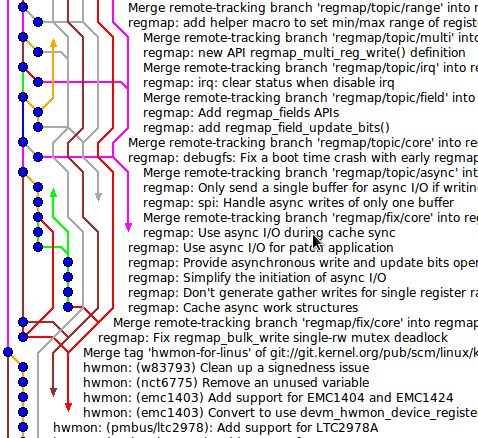
\includegraphics[height=2.5in,width=2.5in]{gitdag.png}
\caption{\small \sl Branching in git DAG for linux kernel development.}
\end{center}
\end{figure}
So it is possible to make a commit months ago from today while several releases may have already been made in the mean time but that commit can belong to any future release. Commits that are being made to a branch may get merged with other branch or the head branch during the release period. This is why we had to track all the way down the trees for each of the 340 releases in the git DAG to find out which commit contributes to which release. We could do this using Git DAG Traversing (GDT) algorithm as shown in Algorithm 1. After applying GDT we collected 381152 out of 400441 commits those are well organized in the git DAG for Linux Kernel development. As we mentioned earlier that we have last couple of release candidates for ``linuxv2.6.12'' and first couple of release candidates for ``linuxv3.12''. We are choping out them because we don't have complete release commit data for version 2.6.12-rc as well as 3.12-rc releases. Out of 400441 commits 19289 are belonging to those releases. So finally we have 381152 commits for 340 releases in our database to progress our work on.

\begin{algorithm}
\caption{GDT: to find Commits within Releases}
\begin{algorithmic}[1]
\REQUIRE
\STATE commit id for all releases
\ENSURE
\FOR{all commits}
\STATE start from new commit, release R
\STATE store commit in ``git\_commit\_release''
\IF{has parent commit}
	\FOR{each parent commit}
		\IF{if parent commit has a release tag}
			\STATE repeat step 1
		\ELSIF{parent commit already stored}
			\STATE compare release versions
			\IF{release version not smaller than R}
				\STATE update existing\_release $\gets$ R
			\ENDIF
		\ELSE
			\STATE store parent commit in ``git\_commit\_release''
			\STATE commit id $\gets$ parent commit id
			\STATE repeat step 3
		\ENDIF
	\ENDFOR
\ELSIF{no parent commit}
	\STATE repeat step 1
\ENDIF
\ENDFOR
\end{algorithmic}
\end{algorithm}

\subsection{Time-Span of Releases}
Another information that we require is what are the durations of the releases of Linux kernel development. To achieve that we joined the table ``git\_refs\_tags'' where all the releases are stored including the splitted release numbers and the table ``git\_commit'' to give us all the dates of commits for each and every releases, so that we can easily find out the duration between two consecutive releases (including release candidates RC). This information will significantly help us because we need to see what is the development period and what are the release periods within a release cycle. We also need to understand how developers are working, what is the impact of their changes made in the code-base during a particular release period later on. Table 1 shows a small portion of this information. Preior to calculate the developers' areas in secion 4.4 we require this information.

\begin{table}[ht]
\caption{Different Releases}  % title of Table
\centering 						% used for centering table
\begin{tabular}{c c c c}				% centered columns (4 columns)
\hline\hline						%inserts double horizontal lines
% table heading
Release & Type & Start Date & End Date \\ [0.5ex]
\hline 							% single horizontal line
% inserting body of the table
linuxv2.6.12-rc2 & rc       & - & 2005-04-16 \\
linuxv2.6.12-rc3 & rc       & 2005-04-16 & 2005-04-20 \\
linuxv2.6.12-rc4 & rc       & 2005-04-20 & 2005-05-07 \\
linuxv2.6.12-rc5 & rc       & 2005-05-07 & 2005-05-24 \\
linuxv2.6.12-rc6 & rc       & 2005-05-24 & 2005-06-06 \\
linuxv2.6.12        & micro & 2005-06-06 & 2005-06-17 \\
linuxv2.6.13-rc1 & rc       & 2005-06-17 & 2005-06-29 \\
linuxv2.6.13-rc2 & rc       & 2005-06-29 & 2005-07-05 \\
linuxv2.6.13-rc3 & rc       & 2005-07-05 & 2005-07-13 \\
...			     & ...	   & ... 		     & ...\\
...			     & ...	   & ... 		     & ... \\
...			     & ...	   & ... 		     & ... \\
linuxv3.11            & minor & 2013-08-25 & 2013-09-02 \\
[1ex]							% adds vertical space
\hline 							% inserts single line
\end{tabular}
\label{table:nonlin} 				% is used to refer this table in the text
\end{table}

Note that the very first row has no information for the ``Start Date'' because we don't have the  complete information prior to stable release ``linuxv2.6.12'' and we have chopped them out. This will not affect our methodology and measurements. From the extraction we found complete records for releases ``linuxv2.6.13'' to ``linuxv2.6.39'' then it is ``linuxv3.0'' to ``linuxv3.11''. Our farther works will be proceeded based on these 39 releases only. As we don't have the complete release information for 3.12 or later as well as for 2.6.12 and earlier ones.

\subsection{Calculate Developers' Area}
Developers are working throughout the release time. Here ``Developers' Area'' means the files developers work in within a release cycle. It doesn't refer to the file itself but it is important to understand which files are being touched by which developers. We see that authors are committing files almost everyday throughout a release but this does not make sure that these commits are going to the next release because commits are being made in different branches and all branches are not supposed to get merged to the next release. We have the commit log data in our hand and we know what is the duration for each and every release (i.e.\ start and end dates). Now it is possible to find out which commits were made for which files by which developer within a certain time range of a release.

A relatively straightforward discipline of Linux Kernel Development team is followed with regard to the merging of patches for each release \cite{linux_kernel}.  At the beginning of each development cycle, the "merge window" is said to be opened.  At that time, code which is deemed to be sufficiently stable (and which is accepted by the development community) is merged into the mainline kernel. The bulk of changes for a new development cycle (and all of the major changes) will be merged during this time, at a rate approaching 1,000 changes ("patches," or "changesets") per day. Strategically linux starts a new kernel release with the merging to get their development branch ready to start development for the next release. So there are two main segments in a release period, one is merge window or merge period (MP) where all the developments works get merged together from different branches. So we can say this is the main development period of a release. A merge period remains opened exactly for two weeks \cite{linux_kernel}, many developers are working in many other branches to develop new features once they are ready to push it to the main kernel then they wait for the upcoming merge window and once it's merge period they all contribute their works for the next release during this Merge Period. Some developers who are mainly responsible to merge new developments verify and accept the new changes and merge them into the main kernel. Another perod in a release cycle is the period of candidate releases which gets opened once the merge window is closed where mainly the bug fixing of minor enhancement works are to be worked on and pushes by small candidate releases. Once all the fixing and enhancements are done for all the codes that had been merged into the main kernel, the release is published. We are calling this period of development as the release period (RP) because no new feature development works do not get accepted during this time, it is just the period prior to publishing a new release.

\subsubsection{Developers' Area in a Merge Period}
Merge Perid can be determined from the previous release date (of any of major, minor or micro releases) to the date of rc-1 (i.e.\ date of the first candidate release). For example if the date of release for ``linuxv2.6.12''  is 2005-06-17 and date of pushing the rc-1 for the next release ``linuxv2.6.13'' is 2005-06-29 then this time period of of 12 days is going to be being called the merge window. Thousands of commits get pushed in the main branch during this period. Table 2 shows merge periods of some releases.

\begin{table}[ht]
\caption{Release Merging Periods}  % title of Table
\centering 						% used for centering table
\begin{tabular}{c c c c}				% centered columns (4 columns)
\hline\hline						%inserts double horizontal lines
% table heading
Release 			& Start Date		& End Date \\ [0.5ex]
\hline 							% single horizontal line
% inserting body of the table
linuxv2.6.13		& 2005-06-17	& 2005-06-29 \\
linuxv2.6.14		& 2005-08-28	& 2005-09-12 \\
linuxv2.6.15		& 2005-10-27	& 2005-11-11 \\
linuxv2.6.16		& 2006-01-02	& 2006-01-17 \\
linuxv2.6.17		& 2006-03-20	& 2006-04-02 \\
linuxv2.6.18		& 2006-06-17	& 2006-07-06 \\
linuxv2.6.19		& 2006-09-19	& 2006-10-04 \\
linuxv2.6.20  		& 2006-11-29	& 2006-12-13 \\
linuxv2.6.21		& 2007-02-04	& 2007-02-20 \\
linuxv2.6.22		& 2007-04-25	& 2007-05-12 \\
linuxv2.6.23		& 2007-07-08	& 2007-07-22 \\
linuxv2.6.24		& 2007-10-09	& 2007-10-23 \\
linuxv2.6.25		& 2008-01-24	& 2008-02-10 \\
[1ex]							% adds vertical space
\hline 							% inserts single line
\end{tabular}
\label{table:nonlin} 				% is used to refer this table in the text
\end{table}

We have the commits contributed to releases and every record explains us who committed the file when did this get churned. If we run an SQL query then we can easily find out for every author and for every particular file how many times a it has been committed by an author and how many churns (addition + deletion = churn) developer has made. We calculate developers' working areas and store the information into a table. A part of that table is shown in table 3.

\begin{table}[ht]
\caption{Developers' Areas in Merge Period}  % title of Table
\centering 						% used for centering table
\begin{tabular}{c c c c}				% centered columns (4 columns)
\hline\hline						%inserts double horizontal lines
% table heading
Author		& File Path			& Commits		& Churn \\ [0.5ex]
\hline 							% single horizontal line
% inserting body of the table
D. S. Miller	& include/.../pci.h		& 1				& 8 \\
V. Hanquez	& arch/.../cpu.c		& 1				& 14 \\
A. Bunk		& drivers/.../shmem.c	& 1				& 2 \\
J. Juhl		& arch/.../generic.c		& 1				& 3 \\
[1ex]							% adds vertical space
\hline 							% inserts single line
\end{tabular}
\label{table:nonlin} 				% is used to refer this table in the text
\end{table}

In this table we see in a merge period within a release cycle D. S. Miller has made change in pci.h file only once where he has made 8 churns. In the similar approach we calculate developers' areas in release period and also for merge period.

\subsubsection{Developers' Areas in Release Period}
As like merge period we can extract developers working in code files during release period. Release Period here in Linux Kernel development process is being considered as since the date of rc1 release (i.e.\ first release candidate opening the gate for the development of the next release) to the date of the next stable release. For example if the date of rc1 for ``linuxv2.6.13'' after releasing ``linuxv2.6.12'' is 2005-06-29 and the date of publishing the release ``linuxv2.6.13'' is 2005-08-28 then we are calling this 60 days of development period for the release as the Release Period. Table 4 is showing some development periods of different releases.

\begin{table}[ht]
\caption{Release Periods}  % title of Table
\centering 						% used for centering table
\begin{tabular}{c c c c}				% centered columns (4 columns)
\hline\hline						%inserts double horizontal lines
% table heading
Release 			& Start Date		& End Date \\ [0.5ex]
\hline 							% single horizontal line
% inserting body of the table
linuxv2.6.13		& 2005-06-29	& 2005-08-28 \\
linuxv2.6.14		& 2005-09-12	& 2005-10-27 \\
linuxv2.6.15		& 2005-11-11	& 2006-01-02 \\
linuxv2.6.16		& 2006-01-17	& 2006-03-20 \\
linuxv2.6.17		& 2006-04-02	& 2006-06-17 \\
linuxv2.6.18		& 2006-07-06	& 2006-09-19 \\
linuxv2.6.19		& 2006-10-04	& 2006-11-29 \\
linuxv2.6.20  		& 2006-12-13	& 2007-02-04 \\
linuxv2.6.21		& 2007-02-20	& 2007-04-25 \\
linuxv2.6.22		& 2007-05-12	& 2007-07-08 \\
linuxv2.6.23		& 2007-07-22	& 2007-10-09 \\
linuxv2.6.24		& 2007-10-23	& 2008-01-24 \\
linuxv2.6.25		& 2008-02-10	& 2008-04-16 \\
[1ex]							% adds vertical space
\hline 							% inserts single line
\end{tabular}
\label{table:nonlin} 				% is used to refer this table in the text
\end{table}

These information above will greatly help us to answer our first couple of research questions and to progress our further works.

\subsection{Finding Code Ownership}
So many developers are working from different development communities throught different development branches. We tried to investigate the "code ownership" \cite{mockus_case_study} evolved in Linux Kernel development. Here code ownership is going to be represented as a percentage of making churns by a developer with respect to the total churns made to a particular file. From the data that we have for complete releases (``linuxv2.6.13'' to ``linuxv3.11'') we found 70210 distinct files that have been churned by developers. We removed those files where no developer made any churn at all during these 39 releases. We investigate the total number of churns for each and every file, we also investigate how many developers contributed for these commits and changes. This information yet does not tell about the ownership, we need to find out ownership for each developer in different development areas in a release cycle. We already have the collection of developers working in merge period and release period within a release cycle and stored them with corresponding files they have worked on, how many commits a developer made to a particular file and how many changes he/she has made. We now update those information with the ownership information. Equation 1 is the base for calculating ownership.
\begin{equation}\omega=\frac{n}{N}*100\end{equation}
Where $\omega$ is the ownership and n is the number of total changes made by an atuthor of a file, N is the total number of changes made for a particular file.
To determine a developer be a owner of a file we are considering that if the developer makes changes more than 80\% of the total churn that has been made by all contributors so far for that file, then that developer can be called as a owner of that file, similarly as C. Gutwin did \cite{gutwin_awareness} for finding out the main developers' group for a project. We calculate code ownership for both Merge Period and Release Period. We also canculate general ownership for all the developers for all the files they have worked ever. Table 6 represents a part of the data which shows the ownerships of the developers in each release cycle.

\begin{table}[ht]
\caption{Code Ownership in RP}  % title of Table
\centering 						% used for centering table
\begin{tabular}{c c c c}				% centered columns (4 columns)
\hline\hline						%inserts double horizontal lines
% table heading
Author 				& Linuxv		& Path				& $\omega$ (\%) \\ [0.5ex]
\hline 							% single horizontal line
% inserting body of the table
Thomas Gleixner		& 2.6.24		& .../numa\_64.h	& 0.0000\\
Jeff Kirsher			& 3.1		& .../ethtool.c		& 0.0000\\
Sathya Perla			& 2.6.29		& .../hwlib.h		& 100.00\\
Roel Kluin			& 2.6.24		& .../innovator.h 	& 100.00\\
David S. Miller		& 2.6.24		& .../visasm.h 		& 100.00\\
Stephen Hemminger	& 2.6.24		& .../qla3xxx.c	 	& 12.083\\
Randy Dunlap			& 2.6.24		& ...\_core.c 		& 100.00\\
[1ex]							% adds vertical space
\hline 							% inserts single line
\end{tabular}
\label{table:nonlin} 				% is used to refer this table in the text
\end{table}
The example given above is calculated for finding ownerships of developers worked for different files in different releases. Ownership is calculated for all the developers in release periods as well as in merge period. In addition we have calculated which file is owned by which developer and also the percentage of working with owned files during merge meriod and release period seperately. These extractions will help us drawing the results from our findings to answer our 3rd and 4th research questions.

\section{Results}
In this section we present results from several quantitative analysis of the archival data from the Linux Kernel development project. The measures we derive from these data are well-suited to answer our research questions.

\textit{What is the release process used by the project?}

In the early 1990's the Linux kernel development was not so busy affair \cite{linux_kernel}. There were very small number of users and developers involved at that time. Developers use a loosely time-based release process. Linux publishes it's major kernel release in every two or three months. If we look at figure 2 the upper Line represents how the stable releases are going on since 2005. From the figure we can see the average duration of each stable release is 62.47 although ``linuxv2.6.24'' was significantly hight as exception, it took 92.8 days. The bottom line which is much steady than the upper one is representing the durations of merge period in each stable release. If we put the releases in a time domain we can see a picture shown in figure 3 where we see that the stable releases are all going on maintaining almost a similar frequency and similar pattern. The highest picks are the merge periods then the smaller picks between the highest ones are representing the rc releases. For more clear view we have plotted only 100 releases of all 340 releases including rc candidates.

Linux Kernel development uses Rolling Release Development Model. Usually every micro release (ex.\ linuxv2.6.x) is a major kernel release with new features, internal API changes, and more. A minor release (ex.\ linuxv3.11) can have around  10 thousand changesets with several hundred thousands of churned lines of  codes (LOC). At the beginning of each stable release the merge window i.e.\ merge period gets opened and all the accepted and stable codes from the community are merged having around 1000 of churns everyday. Merge period approximately for 14 days as shown in the figure 2. The bottom line is representing the merge windows of every releases. We don't have the merge period data for the very first one that's why it's starting from 0.

After getting all the major works merged development period for the next release is announced to be opened. If the next release is going to be linuxv2.6.14 then the release pushed at the end of the merge window will be called linuxv2.6.14-rc1. \textbf{-rc1} release indecates that the time to stabilize the next kernel has begun. These candidate releases continu to be pushed for once a week. If there is any bug fix or any high-priority change only then that goes to the main line during this period. With the continuous rc releases when the new kernel seems to be stable then the it goes for the stable release. Again after the core features are pushed to the main line, merge window gets opened and accepts all other feature developments, patchsets from other branches.

\begin{figure}
\begin{center}
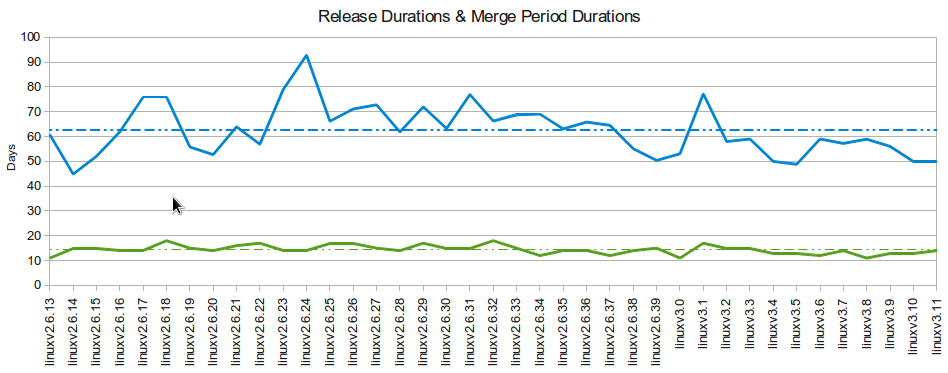
\includegraphics[height=1.7in,width=3.4in]{linxrelmergfreq.png}
\caption{\small \sl Durations of Merge Window and Release Cycle}
\end{center}
\end{figure}

\begin{figure}
\begin{center}
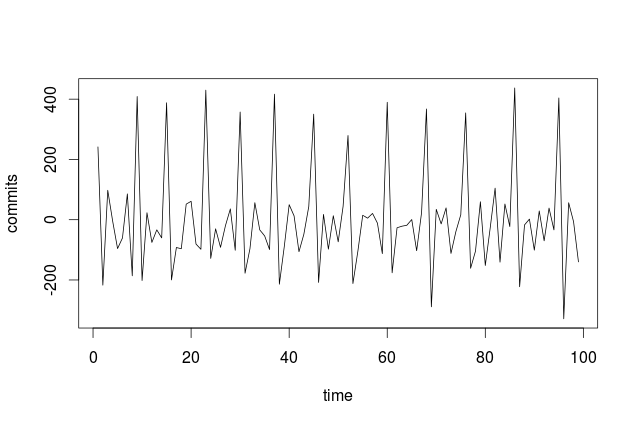
\includegraphics[height=1.7in,width=3.4in]{relTimeDomain100.png}
\caption{\small \sl Time Domain for Releases}
\end{center}
\end{figure}

As a summary, the description above helps to address some of the questions about how Linux Kernel development is organized. Answer to this first research question provides essential background for understanding our quantitative results. We will look into more detail of the development process, distribution of developers among the release segments as well as will try to find answers for our other research questions in the next sections.

\subsection{Difference between release segments}
\textit{How many developers are allocated troughout different segments of a release period? What significant differ-ence can be observed between the segments of an entire release period?}

In order to see how many developers contribute to the new featcher developments and how many contribute in merging and fixing, review and accepting codes from the community during the merge period, we observed the developers' area in Merge Period and developers' area in Release Period. Out of all 381152 commits belonging to all 340 releases 292926 commits were made during the time of merge period which is 76.85\% (more than 2/3) of the total. These commits were made by 14621 individual developers. We now keeping only the records belong to release 2.6.13 to 3.11 because we have complete information for thse releases, so we had to remove the commit records belong to linuxv2.6.12 and linuxv3.12 and later. 11209 developers work in merge period and 7625 developers work around the release period.

In figure 4 we see the boxplot showing that a very large number of developers contribute during the merge period which is in a sense the main development period because all the development branches get merged together during this time, all the new features come into the main branch of the kernel. In release period significantly small number of developers work and this number looks pretty steady for all the releases only a couple of high number appeared in two releases as we see in figure 4. The number of contributions during the main development period over releases looks going up in an increasing manner as shown in figure 5. On the other hand the bottom line for the release developers is pretty steady for all the releases.

\begin{figure}
\begin{center}
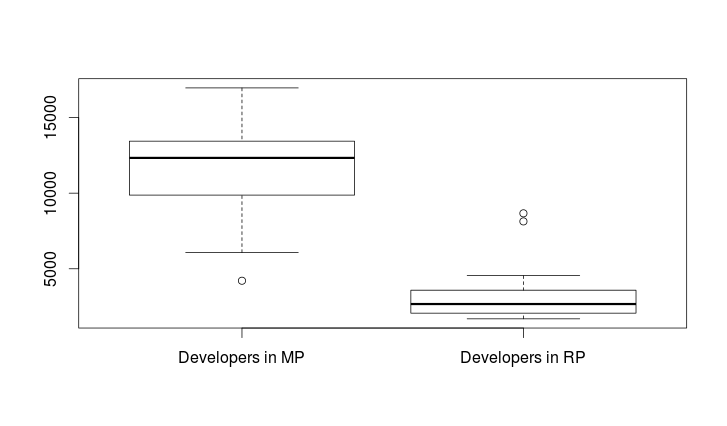
\includegraphics[height=1.7in,width=3.4in]{devsMPRPbox.png}
\caption{\small \sl Developers working in MP \& RP}
\end{center}
\end{figure}

\begin{figure}
\begin{center}
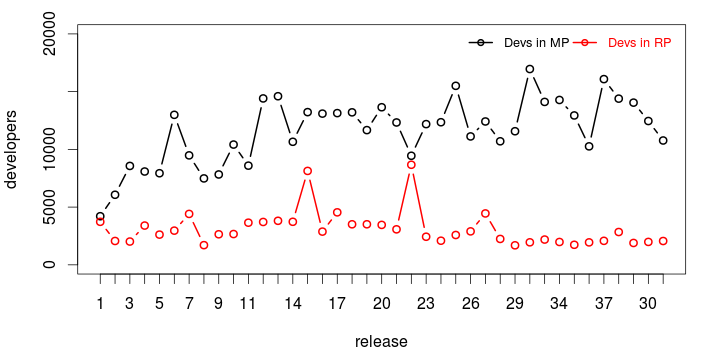
\includegraphics[height=1.7in,width=3.4in]{devsMPRP.png}
\caption{\small \sl Increasing contribution in RDP}
\end{center}
\end{figure}

Once we found different releases and the release periods as well as we calculate the developers' areas and code ownerships for developers we also would like to know what is the difference being created by making changes between the two main segments within an entire release development cycle (i.e.\ Merge Period MP and Release Period RP). To observe this we want to calculate the difference using Jaccard Similarity Coefficient \cite{jaccard_alpine} which is represented by equation 3.
\begin{equation} J(A, B) =\frac{|A \cap B|}{|A \cup B|} \end{equation}
The Jaccard Distance can be obtained by subtracting the Jaccard Coefficient from 1.
\begin{equation} d_j(A, B) = 1 - J(A, B) = \frac{|A \cup B|-|A \cap B|}{|A \cup B|} \end{equation}
Here A and B are two sets. For calculating Jaccard Distance between two releases we are considering the files that have been worked for, in a particular release. If set A is the set of files worked in MP and files worked for in another release is set B then In figure 6 the Jaccard distances between MP and RP for each release can be represented. The average jaccard distance between merge period and release period for all the release cycles is 0.85 and we see the jaccard distance is also going upward by releases except the only exception at release 2.6.34.

\begin{figure}
\begin{center}
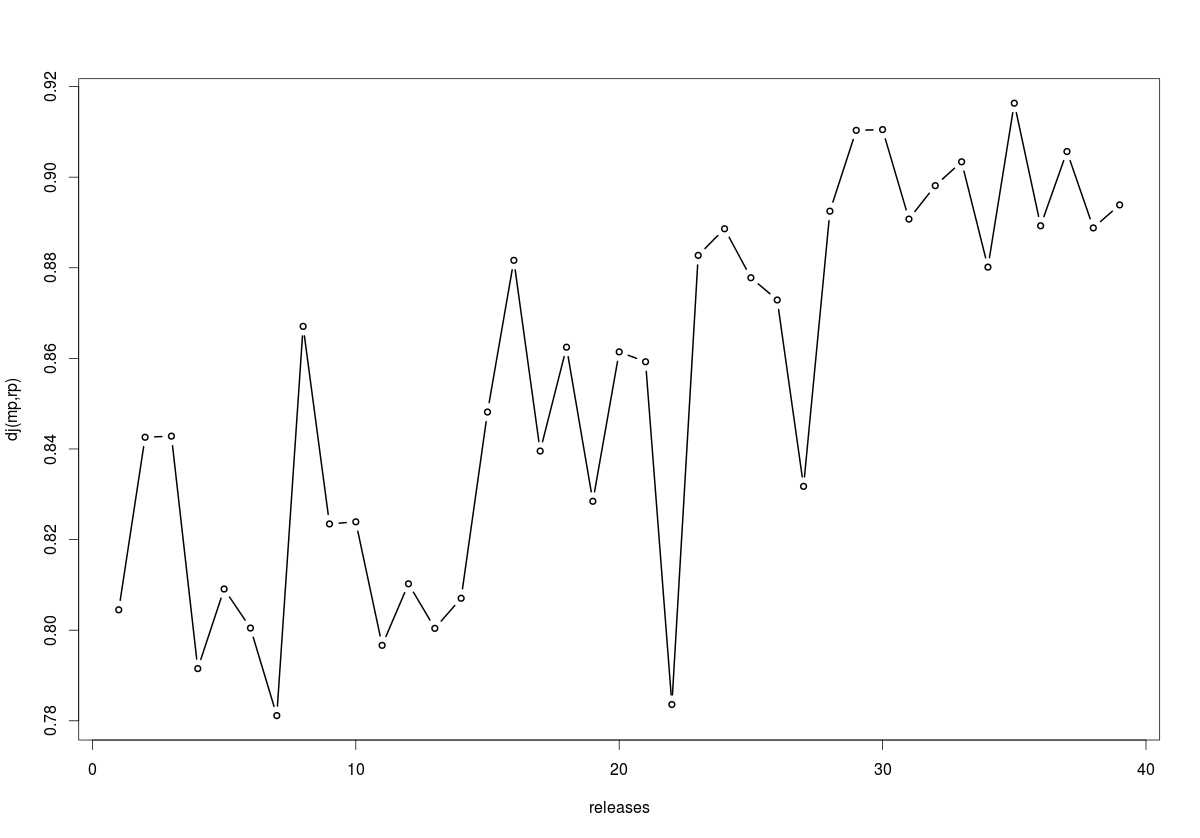
\includegraphics[height=1.7in,width=3.4in]{jdMPRP.png}
\caption{\small \sl Jaccard Distance between the Merge Period and Release Period}
\end{center}
\end{figure}

\subsection{Developers' contributions around the time of release}
\textit{Do developers work on different areas of the system around the time of release?}\newline
\textit{Do developers work in others' code in a high proportion during the rush period?}

We are supposed to find the answers for the two research questions together in this section. Developers work for the software continuously. Some are working for the core development some people are for the fixing and minor enhancements and some for feature developments, planning to merge new features with any up coming release but we would like to understand what number of files they change during the time of development and merging period and how many during the release period. How many of them they really own and how many files they work that they do not own. We also want to know about the code ownership of the developers around the time of release as well as around the time of main development works that get merged during merge meriod.

In order to understand the distribution of the developers around the system we also found that during these release periods 11209 developers have experience of working in the merge meriod and 7625 developers worked in the release period as we already mentioned earlier but we noted that 4908 developers contribute in both merge period and the release period that means near about half (43.78\%) of the developers work during the merge period are shared that means they work for core developments and also bug fixing or minor enhancement works. Figure 7 representing the venn diagram.
\begin{figure}
\begin{center}
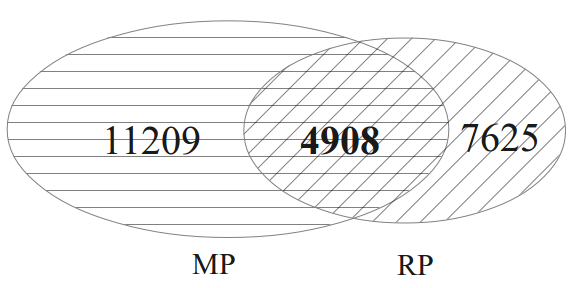
\includegraphics[height=1.3in,width=2.3in]{devDistMPRPvenn.png}
\caption{\small \sl Developers' Distribution in Merge Period and Development Period}
\end{center}
\end{figure}

From release ``linuxv2.6.13'' to ``linuxv3.11'' We examine the contribution in writing code by the developers to understand the behaviour during the two vital segments in a release cycle. Figure 8 plots the cumulative representation of the percentage of working with owned files ($\omega$\textit{MP}) during the merge period and the percentage of working with owned files ($\omega$\textit{RP}) during release period of ``linuxv2.6.13''. From the figure It can be observed that with the increase of every 10 files that developers working in, $\omega$\textit{RP} is going down apart from the line of $\omega$\textit{MP}. Up to a certain number may be around 2200 files developers mostly work with owned files. We see the similar picture for other releases too.
\begin{figure}
\begin{center}
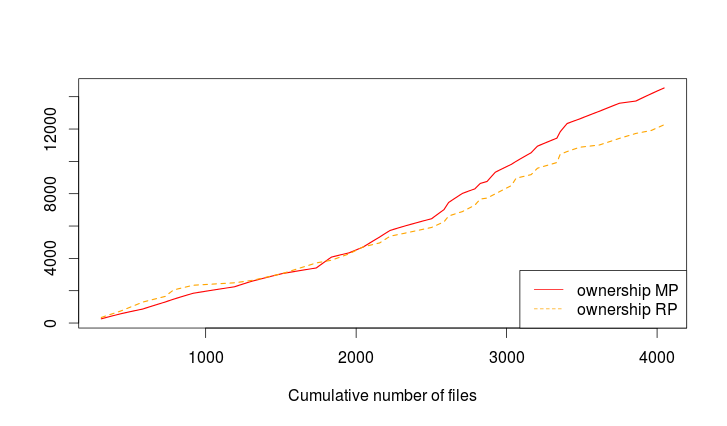
\includegraphics[height=1.7in,width=3.4in]{cumulFileOwnP.png}
\caption{\small \sl Cumulative percentage of working with owned files in MP and RP of release 2.3.13}
\end{center}
\end{figure}

If we simply compare the percentage of working in owned files during merge period ($\omega$\textit{MP}) and the percentage of working in owned files during release period ($\omega$\textit{RP}) for each developer then we see a significant difference of the mean lines as shown in figure 9. In release period developers work with less number of files that they own.

So we can say that in Linux Kernel development developers work in more unfamilier files during the release period. Before the release period main development works are accepted from different branches and they get merged together with main kernel, so, core feature developers finishes their duty for a particular feature development for a particular release within the time of merge period althoug some contributors still work during the release period where basically they work on fixing, testing and minor enhancement related work on the codes that have been merged and accepted from various developers from other branches. It is clear now that during the release period developers work mostly on others' works, the proportion of working with owned files is lower around the release than the proportion during normal development time. When they feel the confidence that everything is tested and can be pushed out for the release, they publish the stable release.

\begin{figure}
\begin{center}
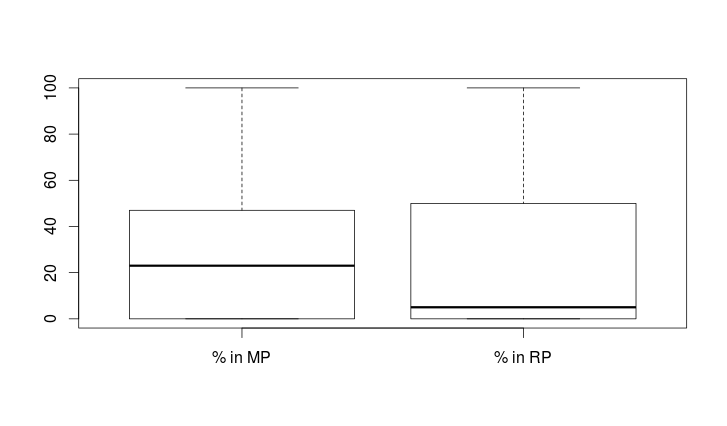
\includegraphics[height=1.7in,width=3in]{ownpMPRPbox.png}
\caption{\small \sl Percentage of working in owned files during Merge Period and Release Period}
\end{center}
\end{figure}

So, finally we can say that in merge periods developers work in more native codes while during the regular release development period the percentage of working with native code is very low in number although this percentage of working in owned code during merge period does not significantly relate to other co-factors.

\subsection{Time for commits to go live}
\textit{How long a commit take to get pushed into the main kernel? Does it differ in different periods of release?}

There are thousands of commits goes to the main kernel during the merge meriod. All they are to be considered as the normal development commits or regular development or core development commits for developing new features to the kernel. Merge period remains opened for two weeks only, the development works that are supposed to go for a particular release are not developed during this couple of weeks. These have been developed since many days ago on a different development branch by any developer. For a particular feature that is going to the current release there are hundreds of commits, obviously all these commits are not made during the merge period of the current release 90-100\% commits must have been made before the opening of the merge period of current release. As described in section 4.3, we have sorted up the releases according to the git DAG. This helps us to calculate how many days in past the first commit of this particular feature had been made which is going to be pushed into the current release. The duration a commit was made to the local branch to the date it is pushed into the main branch is being called here ``lag'' of commits. Figure 10 represents lag of the commits made for regular development and lag of the commits made during the release period.

\begin{figure}
\begin{center}
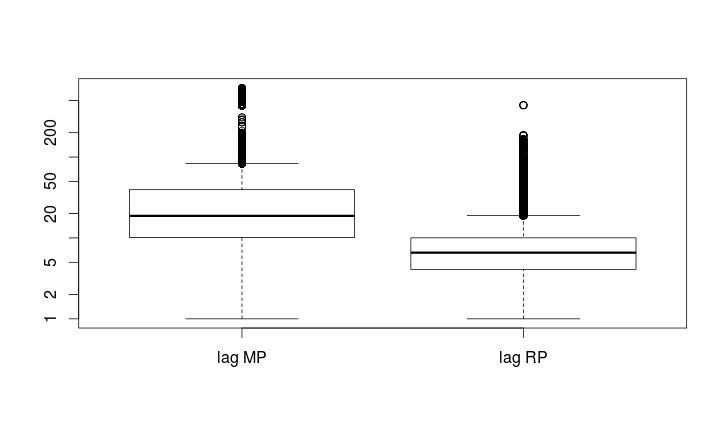
\includegraphics[height=1.7in,width=3in]{lagMPRPbox.png}
\caption{\small \sl Time takes for development commits and commits around release periods to get released}
\end{center}
\end{figure}

From figure 10 we can understand it easily that rather quick fixes are made during the release period. With the small sets of bug fixes, important wuick enhancements candidate releases are pushed and once the kernel seems to me more stable with all the new features that's been merged at the beginning of the release cycle, stable release is published. Comperatively lag for the feature development commits is quite high. Median for the lags for the commits during this time is 5.57 while median for the lags for the commits goes to the main kernel during merge period is 26.15 which is a significant different between these two periods of a release cycle.

\subsection{Developers' focus on code-base around the time of release}
\textit{Are there certain areas of the system that receive increased attention (i.e.\ do developers focus on a smaller set of files around releases)?}
Answer to the following questions are going to be looked for to answer this research question:
\renewcommand{\labelenumi}{q\theenumi:}
\begin{enumerate}
\item{How many times a file has been committed during merge period?}
\item{How many authors made those commits?}
\item{How many churns were made to the files during each commit?}
\item{What is the time interval for the commits for a file?}
\item{How many files each developer deals with during merge period?}
\item{How many files each developer deals with during release development period?}
\item{What is the jaccard distance J(mp1, rdp1), J(rdp1, rdp0) and J(rdp0, mp1)?}
\end{enumerate}
We found the relation J(mp1, rdp1) > J(rdp1, rdp0) < J(rdp0, mp1) for the minor releases is significant but among the micro stable releases this relation is not significant at all.

\section{Conclusions}
This section will be written at the end.
%\end{document}  % This is where a 'short' article might terminate

\bibliographystyle{abbrv}
\bibliography{paper1} 
\appendix
%Appendix A
\section{Headings in Appendices}
Apendix section will be written later with the following subsections may be:
\subsection{Introduction}
...
\subsection{Background and Motivation}
\subsubsection{Related Works}
...
\subsubsection{Methodology and Data}
...
\subsection{Conclusions}
...
\subsection{Acknowledgments}
...

\subsection{References}
... ...

\balancecolumns
\end{document}